\documentclass{article}
\usepackage{graphicx}
% \usepackage[paperheight=16cm,paperwidth=12cm,textwidth=10cm]{geometry}
\usepackage{lipsum}
\usepackage[T2A]{fontenc}
% \usepackage[koi8-r]{inputenc}
\usepackage[utf8]{inputenc}

\graphicspath{ {./Results/} }

\title{Merge Sort}
\author{Dadmo}
\date{\today}

\begin{document}
\maketitle

\section{Plan}
\begin{enumerate}
    \item Merge Sort
    \item Random Lists
    \item Linked Lists
    \item Converters
    \item Comparisions and Results
\end{enumerate}
    \section{Merge Sort}
    MergeSort --- клас, який має реалiзованi 4 варiанти алгоритму сортування злиттям. 
    \begin{enumerate}
        \item Рекурсивний (Top-Down MergeSort)
        \item Ітеративний (Bottom-Up MergeSort)
        \item Ітеративний з оптимiзацiями cutoff(-to-insertion), stop-if-already-sorted, eliminate-the-copy-to-the-auxiliary-array.
        \item Сотування злиттям для зв’язного списку
    \end{enumerate}
    \indent В моїй реалiзації Ітеративного сортування злиттям використовується менше порівнянь для реверсивно відсортованих списків.
    \newline
    \indent В моїй реалiзації Ітеративного сортування злиттям з оптимiзацiями массиви розміру між 80eA та 90eA, де eA --- 10 в степені A, сортуються не до кінця (Останні с елементів) через оптимізацію eliminate-the-copy-to-the-auxiliary-array.
    \newline
    \indent Також реалiзовано порiвняльний аналiз (з даними рiзного розмiру) всiх чотирьох варiантiв
    алгоритму сортування злиттям вiдносно часу виконання, кiлькостi проведених
    порiвнянь, операцiй "копiювань" та використаної пам’ятi. Окрім цього є показ на скільки відстотків обрахунки вже завершено.
    \newline
    % \newline
    \section{Random Lists}
    RandomLists --- клас, який має реалiзованi 5 варiанти генерацiї спискiв.
    \begin{enumerate}
        \item Повнiстю вiдсортований (sorted) --- на вхід подається лише розмiр списку.
        \item Випадковi (random) --- на вхід подається лише розмiр списку.
        \item Майже вiдсортований (almostsorted) --- на вхід подається розмiр списку, та відсоток безпорядку.
        \item Вiдсортованi в зворотному порядку (reverse) --- на вхід подається лише розмiр списку.
        \item Лише з декiлькома рiзними значеннями (somenumbers) --- на вхід подається розмiр списку, та діапазон значень (Початок, Кiнець).
    \end{enumerate}
    \section{Linked Lists}  

        \indent Node --- клас, який зберігає дані, а також посилання на наступний та попередній елементи.
        Для нього реалiзовано отримання розмiру в байтах, а також реалiзованi усі порівняння.

        LinkedList --- клас, який зберігає посилання на перший та останній елементи.
        Для нього реалiзовано отримання розмiру в байтах, а також реалiзоване
        додавання елементів, розширення списку, підрахунок певної підкількості елементів, а також видалення елементів.
        \newline
        \indent Додатково реалiзовано призначення та отримання елемента за індексом, слайсом індексів списку.
    \section{Converters}
    Converter --- клас, в якому реалiзовано конвертацiю масиву у зв’язний список та навпаки.
    \section{Comparisions and Results}
        Подивимося результати виконання. Розміри масивів: від 10 до 10000 елементів з кроком в 100.
        \newline
        \newpage
        \textbf{Спочатку для відсортованих масивів:}
        \newline
        Час виконання:
        \newline
            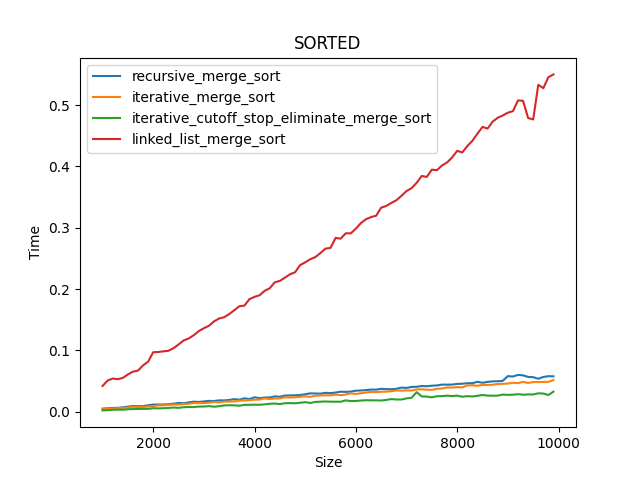
\includegraphics[scale=0.5]{sorted_Time_4_sorts_90_numbers_50.png}
            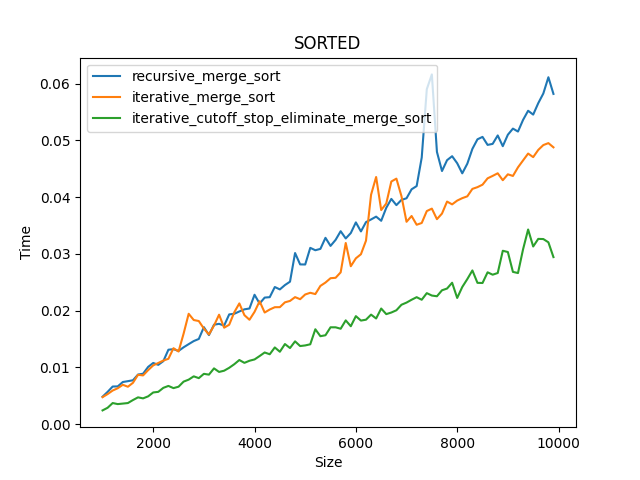
\includegraphics[scale=0.5]{sorted_Time_3_sorts_90_numbers_50.png}
        \newline
        Кiлькiсть проведених порiвнянь:
        \newline
            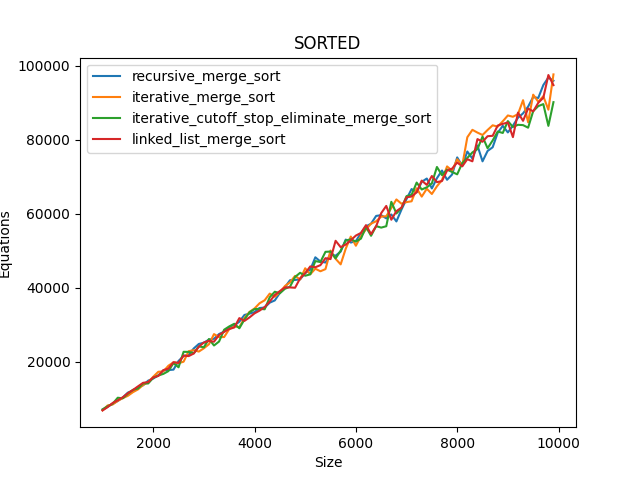
\includegraphics[scale=0.5]{sorted_Equations_4_sorts_90_numbers_50.png}
            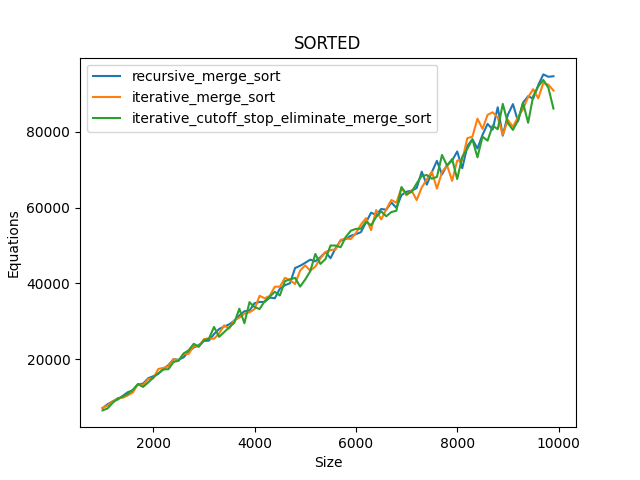
\includegraphics[scale=0.5]{sorted_Equations_3_sorts_90_numbers_50.png}
        \newpage
        Операцiї "копiювань":
        \newline
            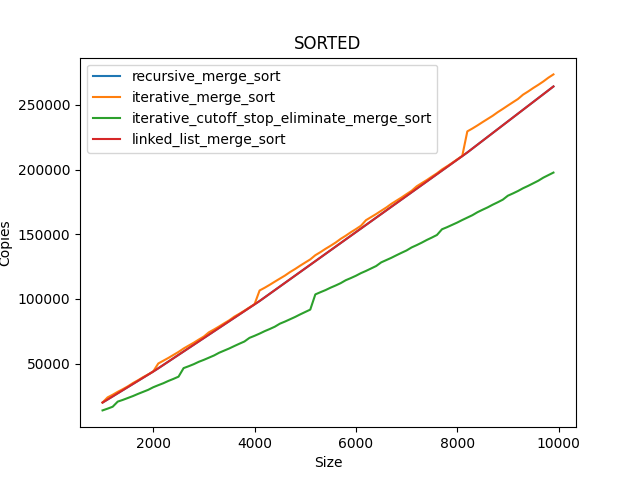
\includegraphics[scale=0.5]{sorted_Copies_4_sorts_90_numbers_50.png}
            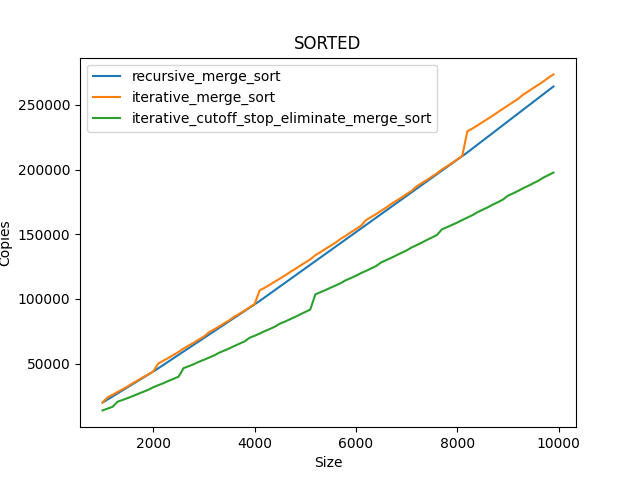
\includegraphics[scale=0.5]{sorted_Copies_3_sorts_90_numbers_50.png}
        \newline
        Використано пам’ятi:
        \newline
            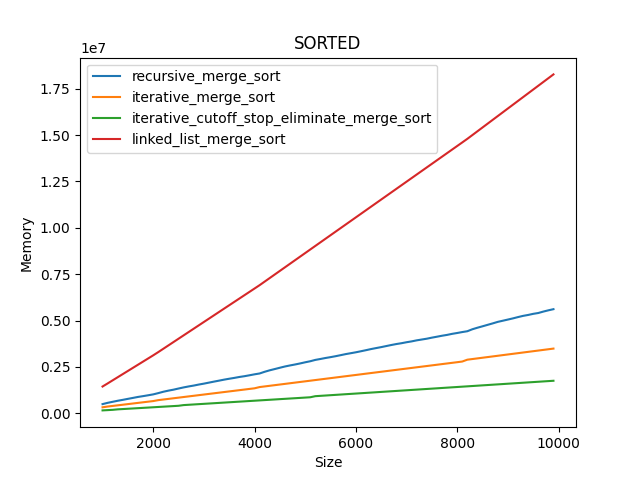
\includegraphics[scale=0.5]{sorted_Memory_4_sorts_90_numbers_50.png}
            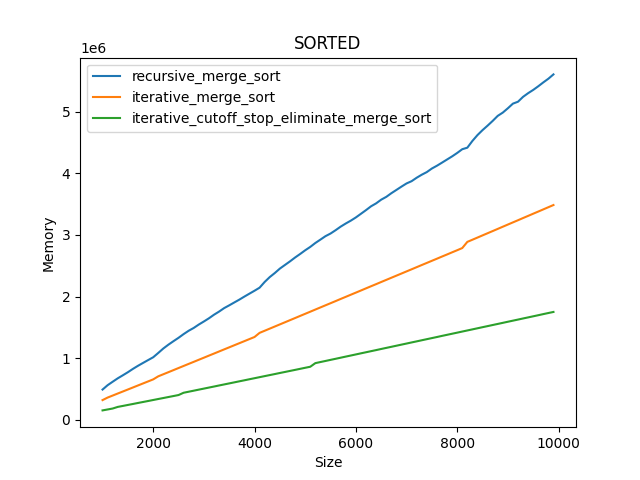
\includegraphics[scale=0.5]{sorted_Memory_3_sorts_90_numbers_50.png}
        \newpage
        \textbf{Потім для масивів випадкових значень:} 
        \newline
        Час виконання:
        \newline
            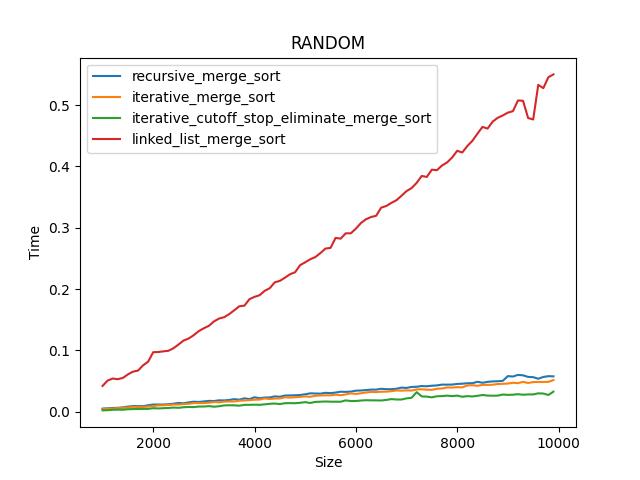
\includegraphics[scale=0.5]{random_Time_4_sorts_90_numbers_50.png}
            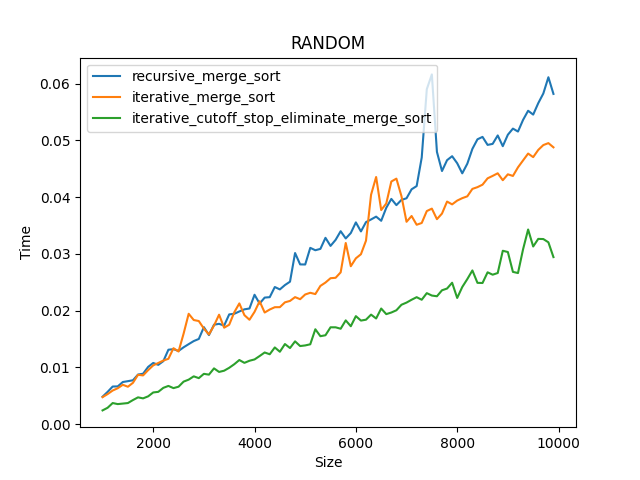
\includegraphics[scale=0.5]{random_Time_3_sorts_90_numbers_50.png}
        \newline
        Кiлькiсть проведених порiвнянь:
        \newline
            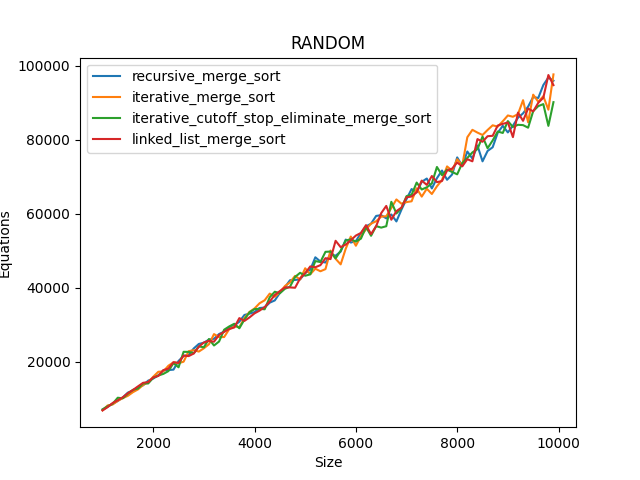
\includegraphics[scale=0.5]{random_Equations_4_sorts_90_numbers_50.png}
            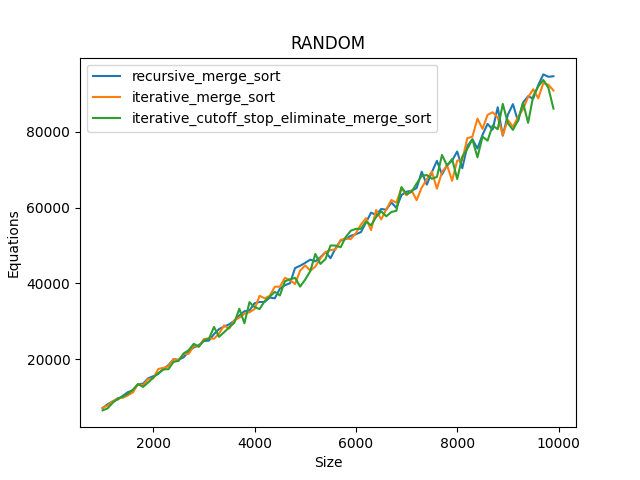
\includegraphics[scale=0.5]{random_Equations_3_sorts_90_numbers_50.png}
        \newpage
        Операцiї "копiювань":
        \newline
            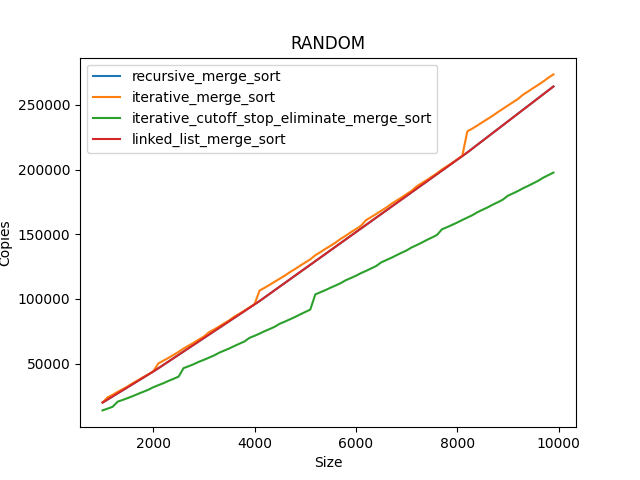
\includegraphics[scale=0.5]{random_Copies_4_sorts_90_numbers_50.png}
            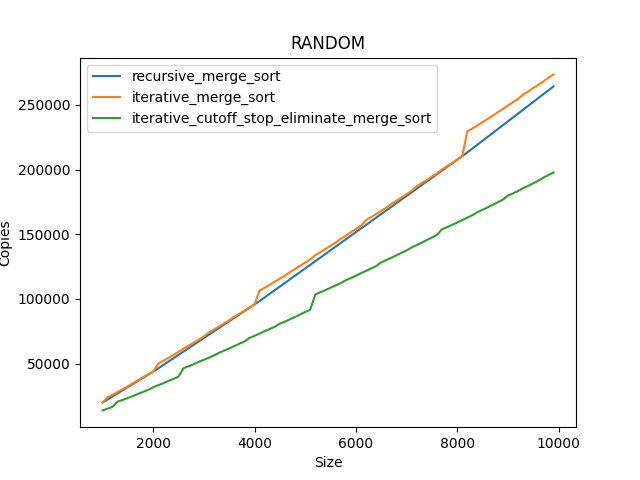
\includegraphics[scale=0.5]{random_Copies_3_sorts_90_numbers_50.png}
        \newline
        Використано пам’ятi:
        \newline
            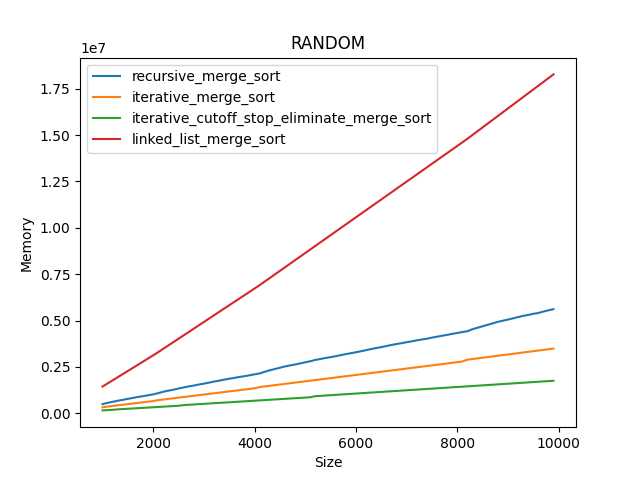
\includegraphics[scale=0.5]{random_Memory_4_sorts_90_numbers_50.png}
            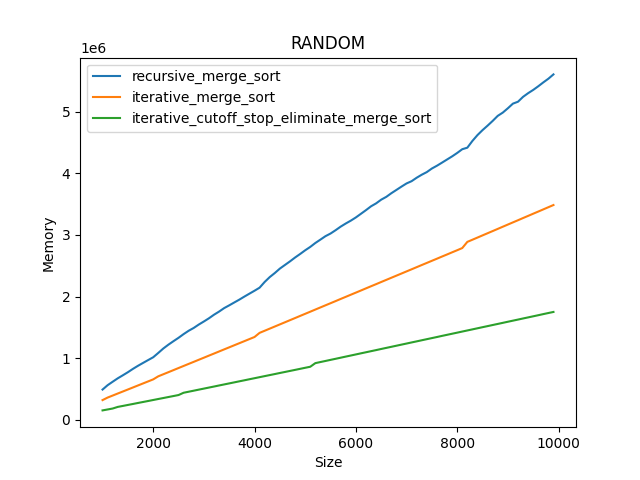
\includegraphics[scale=0.5]{random_Memory_3_sorts_90_numbers_50.png}
        \newpage
        \textbf{Масив майже відсортованих значень:}
        \newline
        Час виконання:
        \newline
            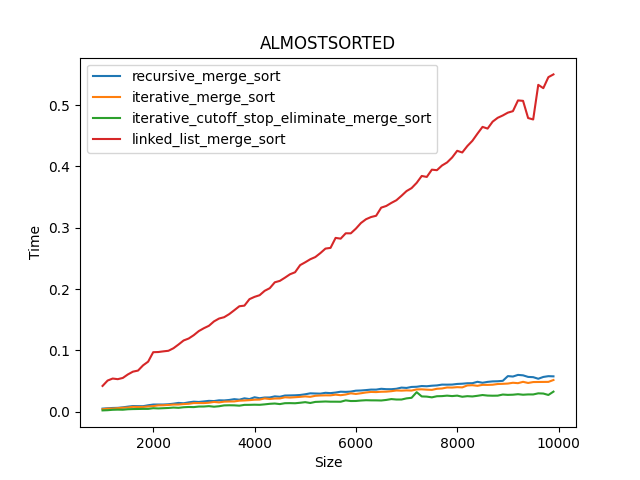
\includegraphics[scale=0.5]{almostsorted_Time_4_sorts_90_numbers_50.png}
            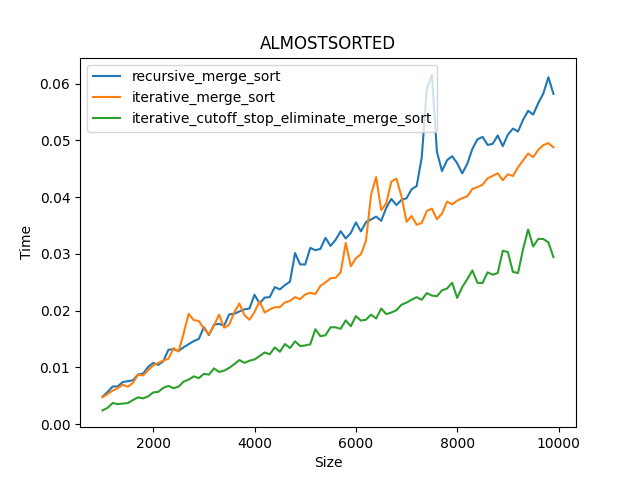
\includegraphics[scale=0.5]{almostsorted_Time_3_sorts_90_numbers_50.png}
        \newline
        Кiлькiсть проведених порiвнянь:
        \newline
            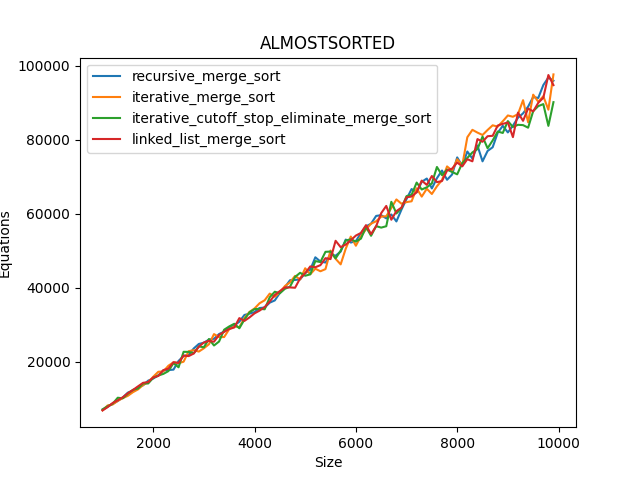
\includegraphics[scale=0.5]{almostsorted_Equations_4_sorts_90_numbers_50.png}
            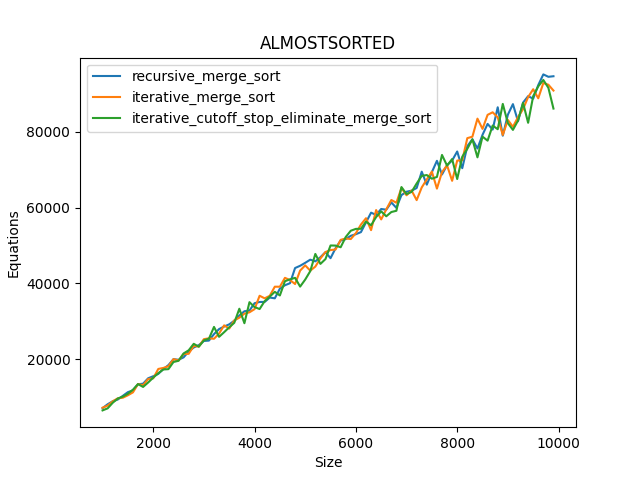
\includegraphics[scale=0.5]{almostsorted_Equations_3_sorts_90_numbers_50.png}
        \newpage
        Операцiї "копiювань":
        \newline
            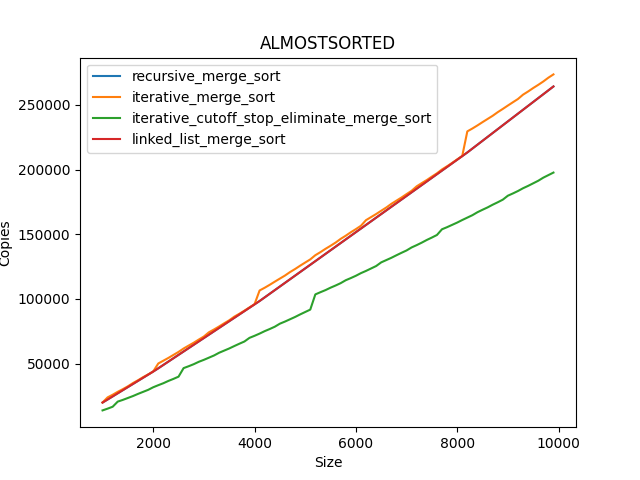
\includegraphics[scale=0.5]{almostsorted_Copies_4_sorts_90_numbers_50.png}
            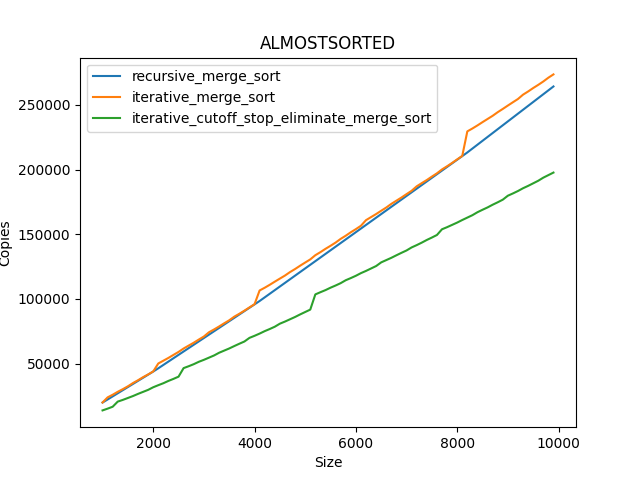
\includegraphics[scale=0.5]{almostsorted_Copies_3_sorts_90_numbers_50.png}
        \newline
        Використано пам’ятi:
        \newline
            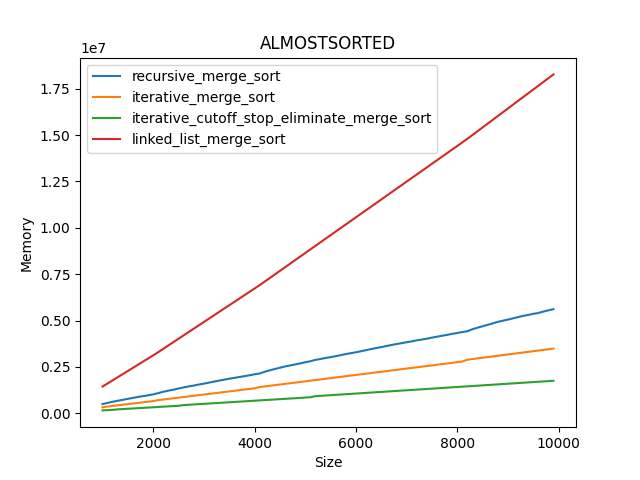
\includegraphics[scale=0.5]{almostsorted_Memory_4_sorts_90_numbers_50.png}
            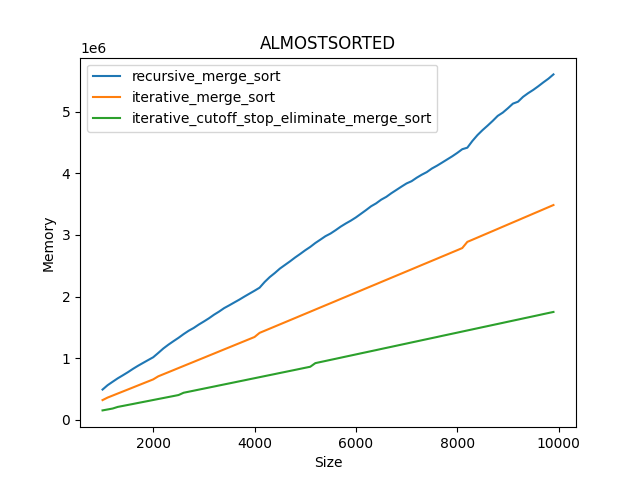
\includegraphics[scale=0.5]{almostsorted_Memory_3_sorts_90_numbers_50.png}
        \newpage
        \textbf{Масив відсортованих значень у зворотному порядку:}
        \newline
        Час виконання:
        \newline
            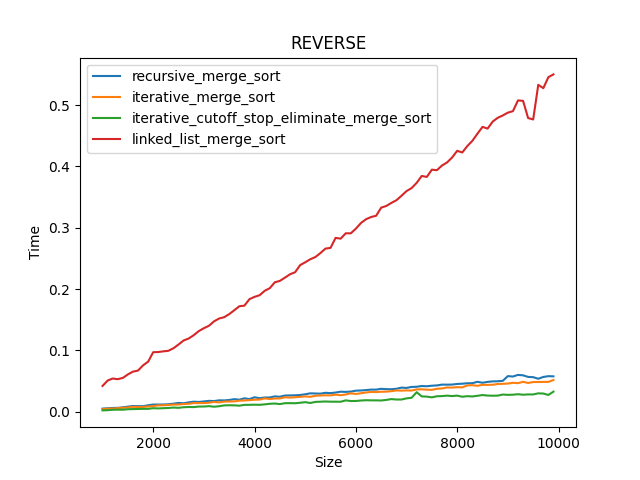
\includegraphics[scale=0.5]{reverse_Time_4_sorts_90_numbers_50.png}
            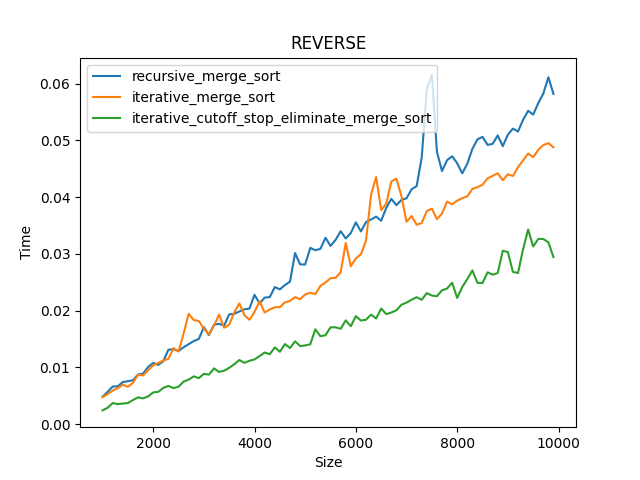
\includegraphics[scale=0.5]{reverse_Time_3_sorts_90_numbers_50.png}
        \newline
        Кiлькiсть проведених порiвнянь:
        \newline
            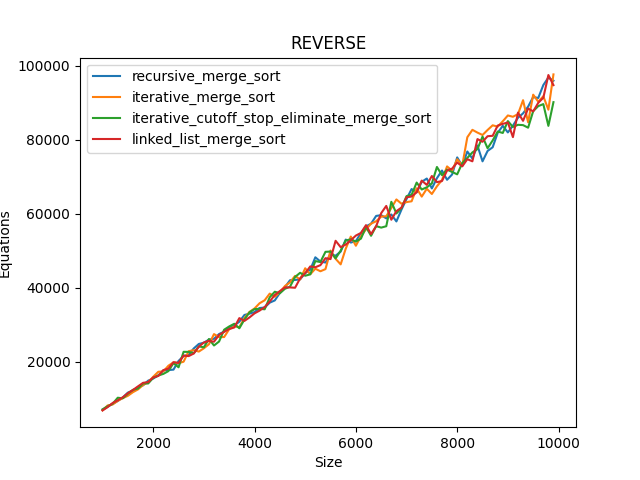
\includegraphics[scale=0.5]{reverse_Equations_4_sorts_90_numbers_50.png}
            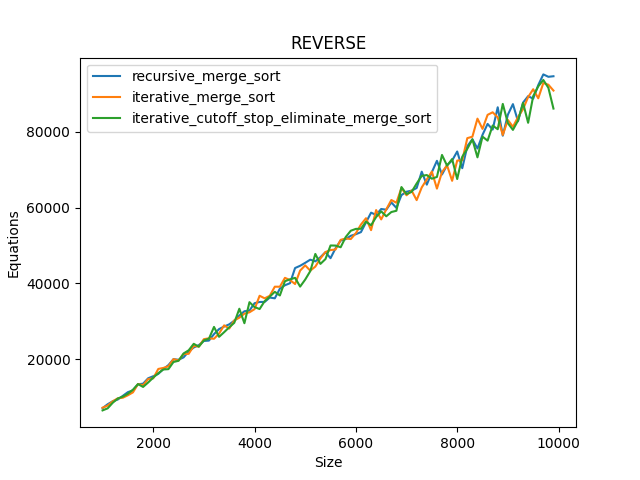
\includegraphics[scale=0.5]{reverse_Equations_3_sorts_90_numbers_50.png}
        \newpage
        Операцiї "копiювань":
        \newline
            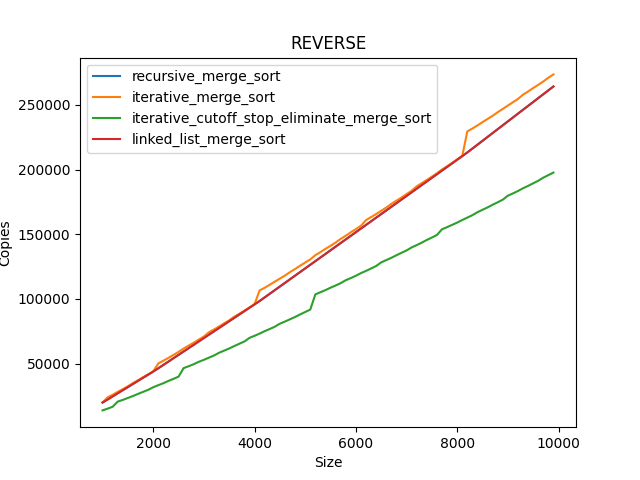
\includegraphics[scale=0.5]{reverse_Copies_4_sorts_90_numbers_50.png}
            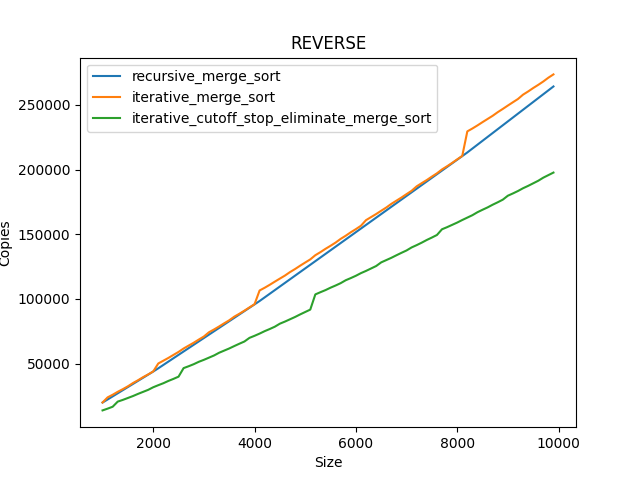
\includegraphics[scale=0.5]{reverse_Copies_3_sorts_90_numbers_50.png}
        \newline
        Використано пам’ятi:
        \newline
            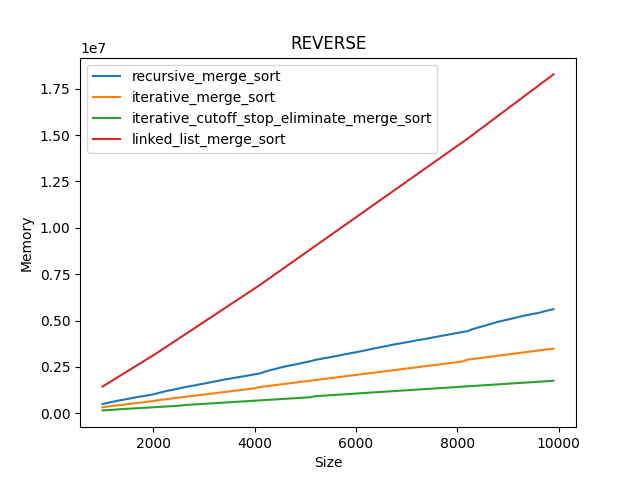
\includegraphics[scale=0.5]{reverse_Memory_4_sorts_90_numbers_50.png}
            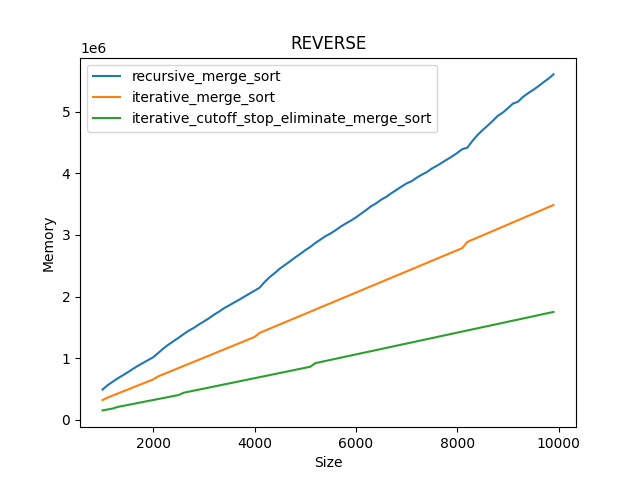
\includegraphics[scale=0.5]{reverse_Memory_3_sorts_90_numbers_50.png}
        \newpage
        \textbf{Масив тільки з декiлькома рiзними значень:}
        \newline
        Час виконання:
        \newline
            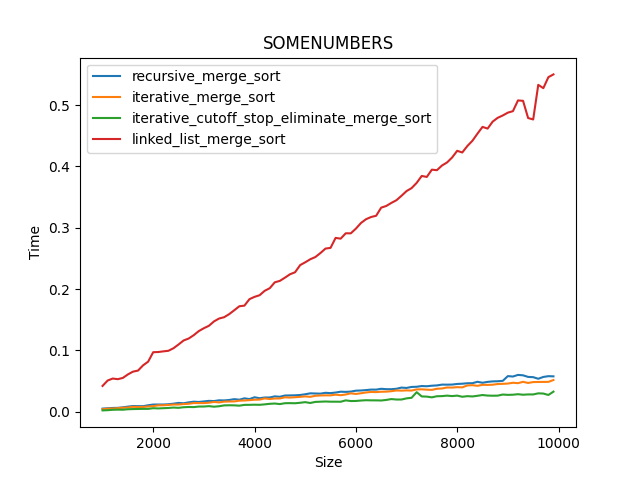
\includegraphics[scale=0.5]{somenumbers_Time_4_sorts_90_numbers_50.png}
            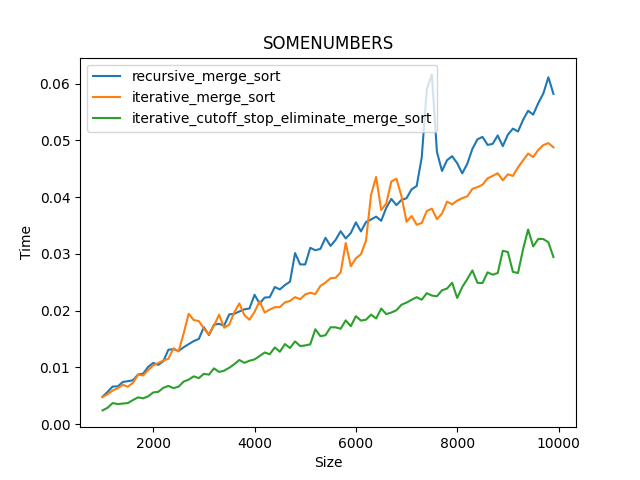
\includegraphics[scale=0.5]{somenumbers_Time_3_sorts_90_numbers_50.png}
        \newline
        Кiлькiсть проведених порiвнянь:
        \newline
            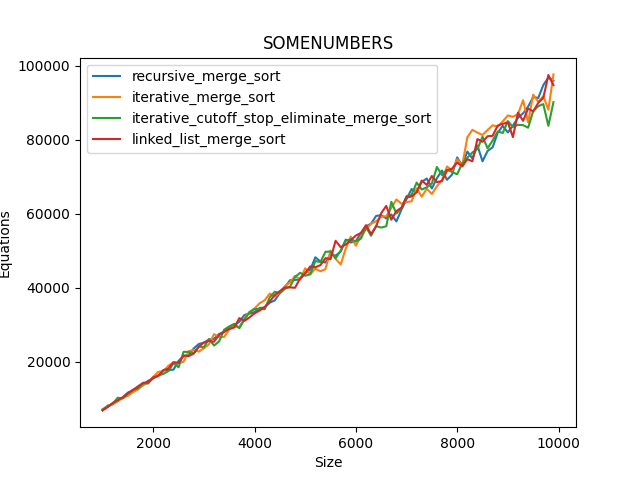
\includegraphics[scale=0.5]{somenumbers_Equations_4_sorts_90_numbers_50.png}
            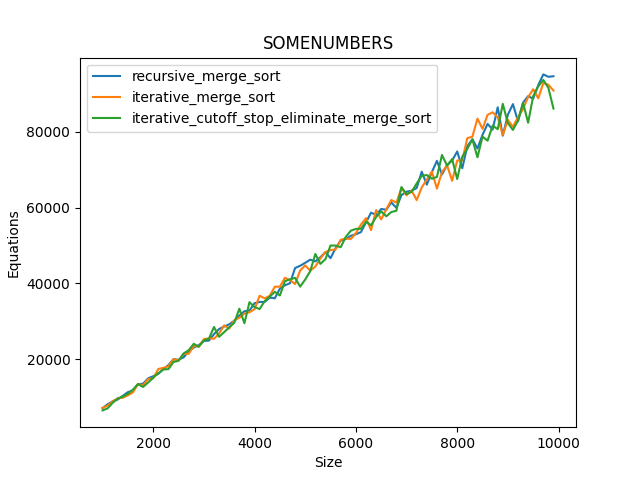
\includegraphics[scale=0.5]{somenumbers_Equations_3_sorts_90_numbers_50.png}
        \newpage
        Операцiї "копiювань":
        \newline
            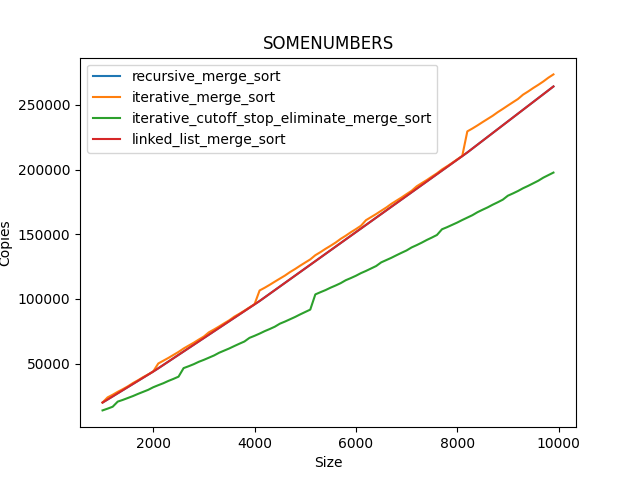
\includegraphics[scale=0.5]{somenumbers_Copies_4_sorts_90_numbers_50.png}
            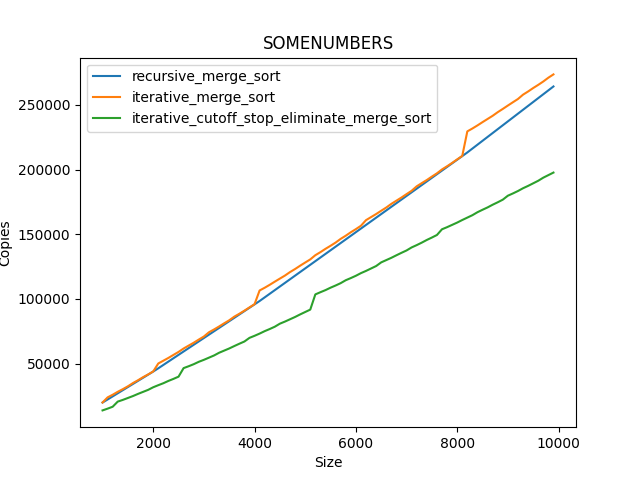
\includegraphics[scale=0.5]{somenumbers_Copies_3_sorts_90_numbers_50.png}
        \newline
        Використано пам’ятi:
        \newline
            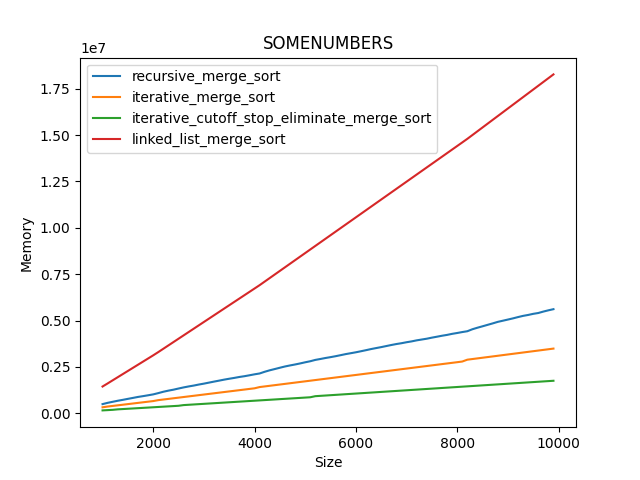
\includegraphics[scale=0.5]{somenumbers_Memory_4_sorts_90_numbers_50.png}
            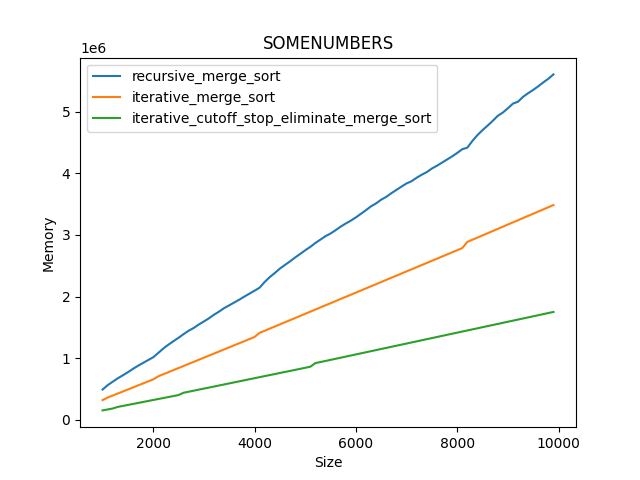
\includegraphics[scale=0.5]{somenumbers_Memory_3_sorts_90_numbers_50.png}
        \newpage
\end{document}

% 4. Оформлення результатiв роботи та звiту
% Результатом роботи є всi тексти програм, за потреби скомпiльованi виконуванi файлi (якi
% мають запускатися на чистiй ОС; якщо є потреба, можна використовувати контейнери), необхiдна
% документацiя щодо використання з прикладами застосування та звiт.
% Звiт до комп’ютерного практикуму оформлюється згiдно зi стандартними правилами
% оформлення наукових робiт. Тексти програм не включати у звiт.